% \subsection{Flatsat}

% Most of the tests were performed on Flatsat (an abbreviation from Flat Satellite), an electronic test bench, which consist of mix of flight models, engineering models of the instruments and Electrical Ground Support Equipment (EGSE). EGSE are the test instruments and/or mocks (fake) instruments, which allow testing without the need for actual hardware.

% PW-Sat2 Flatsat was integrated in Space Research Centre in Warsaw. Flatsat is shown in the figure \ref{TODO}.

% \subsubsection{Flatsat Ground Station mock}
% To perform the communication tests a Ground Station mock was created of flatsat. It was built using to Software-Defined Radios: one, as downlink receiver, same as to be installed in the Ground Station (Funcube Pro+), and the second (PlutoSDR) to generate uplink signals. Use of SDR instead of analogue radio transceiver greatly simplified the tests performed. Ground station mock is shown in the figure \ref{TODO}. 




\chapter{Space segment}
Space segment is a part of the satellite communication system that resides on the satellite itself. It is divided into two main parts: communication subsystem (COMM) and antennas (ANTs) connected with two coaxial cables.

Space segment is critical in system operation and reliability - there is no possibility to carry out any repairs, perform maintenance or adjustment once on orbit. It is exposed to the space environment - wide temperature range, thermal cycling, cosmic radiation and vacuum.

Because of the mentioned requirements it was decided to choose commercially available and flight-proven CubeSat components to increase the overall reliability of the system.

% -----------------------------------------------------------------------------------------------------------
% -----------------------------------------------------------------------------------------------------------
% -----------------------------------------------------------------------------------------------------------

\section{Spacecraft communication transceiver}
\label{section:comm_design}
CubeSat design specification \cite{cubesat_spec}, with which PW-Sat2 is compliant, defines common PC/104 connector, which is the main data bus for all satellite subsystems. On the connector, two \iic and two CAN buses are defined and most of the components are compatible to each other. However, due to the lack of CAN interface on On-Board Computer (CubeComputer from CubeSpace \cite{cubespace_website}) radio should use \iic communication bus.

When the subsystem was ordered (in year \si{2014}), the choice of available products was very limited, and the only radio which was compliant with above mentioned requirements was \texttt{ISIS VHF uplink/UHF downlink Full Duplex Transceiver}. Its view and block diagram is shown in the figures \ref{ISIS_TRXvU_photo} and \ref{ISIS_TRXvU_block_diagram}.

\begin{figure}[H]
    \centering
    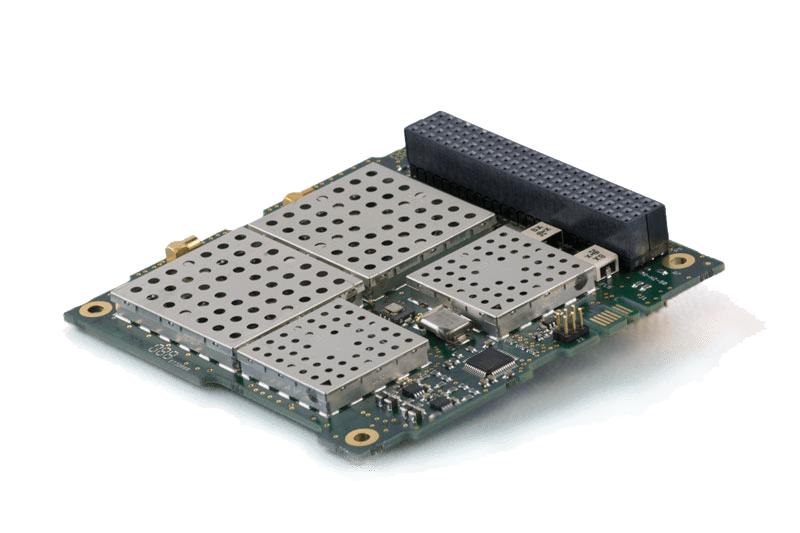
\includegraphics[width=0.5\paperwidth]{img/4/ISIS-radio-UHF-VHF-min.png}
    \caption{ISIS VHF uplink/UHF downlink Full Duplex Transceiver photo. Source: \cite{isis_trxvu}}
    \label{ISIS_TRXvU_photo}
\end{figure}

\begin{figure}[H]
    \centering
    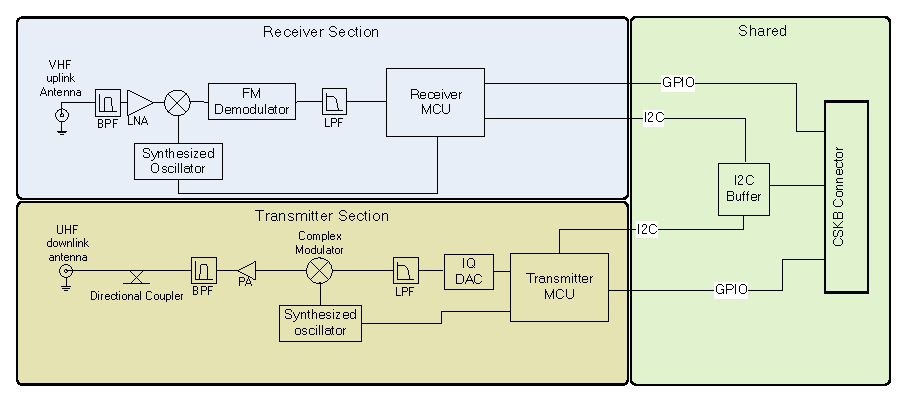
\includegraphics[width=0.8\paperwidth]{img/4/ISIS_TRXvU_block_diagram.eps}
    \caption{ISIS VHF uplink/UHF downlink Full Duplex Transceiver block diagram. Source: \cite{isis_trxvu}}
    \label{ISIS_TRXvU_block_diagram}
\end{figure}

Basic characteristics: \\
\begin{tabular}{c|c}
     \textbf{downlink} & \textbf{uplink} \\ \hline
     \multicolumn{2}{c}{dual-\iic communication standard} \\
     \multicolumn{2}{c}{AX.25 frame format} \\
     \si{430}-\SI{450}{\MHz} frequency range & \si{140}-\SI{150}{\MHz} frequency range \\
     \SI{0.5}{\watt} downlink power & \SI{-98}{\dBm} sensitivity for \si{10^-5}~BER \\
     \si{1.2} - \SI{9.6}{\kilo\bit / \second} bitrate & \SI{1.2}{\kilo\bit / \second} bitrate \\ 
     BPSK modulation with G3RUH scrambling & FM-modulated AFSK \\ 
\end{tabular}

Transceiver was tested separately for its uplink and downlink capabilities. Tests are critical to make sure that radio parameters are maintained in the system, and to verify manufacturers' data.

\subsection{Sensitivity measurement}
Sensitivity was measured by the setup shown in the figure \ref{4_uplink_sensitivity}. Test procedure:

\begin{itemize}
    \item measuring output power of PlutoSDR using spectrum analyzer with wide RBW filter (\SI{1}{\MHz}),
    \item calculating input power to the Communications module,
    \item PER is calculated by transmitting data frames using PlutoSDR (with GNUradio) and receing them by On-Board Computer connected to the PC,
    \item decreasing output power of PlutoSDR and measuring PER for each point (\si{1000}~frames).
\end{itemize}

\begin{figure}[H]
    \centering
    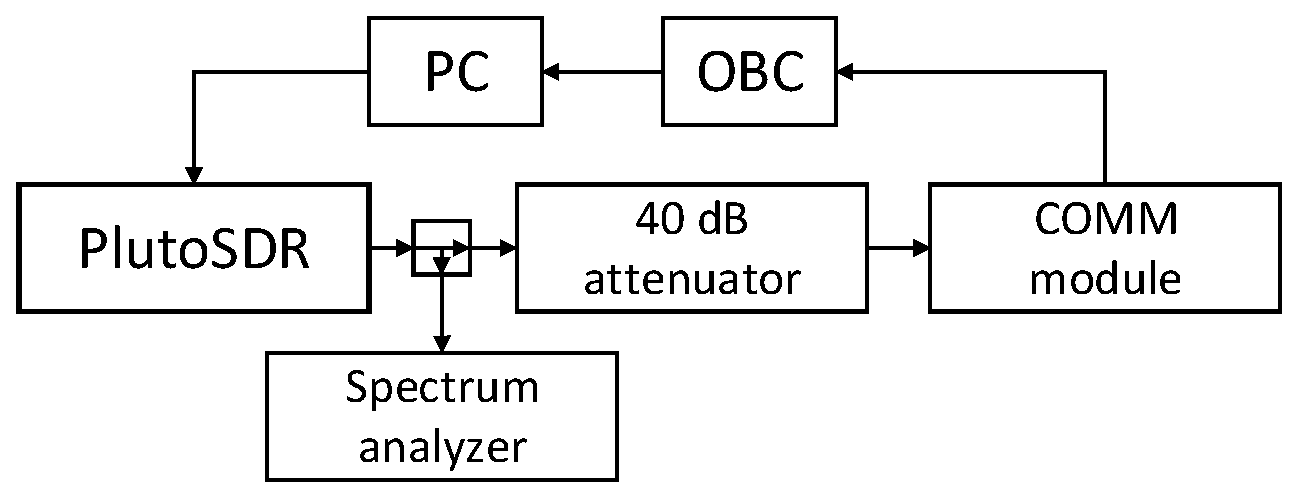
\includegraphics[width=0.6\paperwidth]{img/4/uplink_sensitivity.eps}
    \caption{Uplink sensitivity measurement block diagram.}
    \label{4_uplink_sensitivity}
\end{figure}

Measured PER chart is shown in the figure \ref{4_uplink_sensitivity_graph}. It is compared to the ideal BFSK curve. For usable PER of about \SI{1}{\percent} the sensitivity of the communication module is \SI{-95}{\dBm}.

\begin{figure}[H]
    \centering
    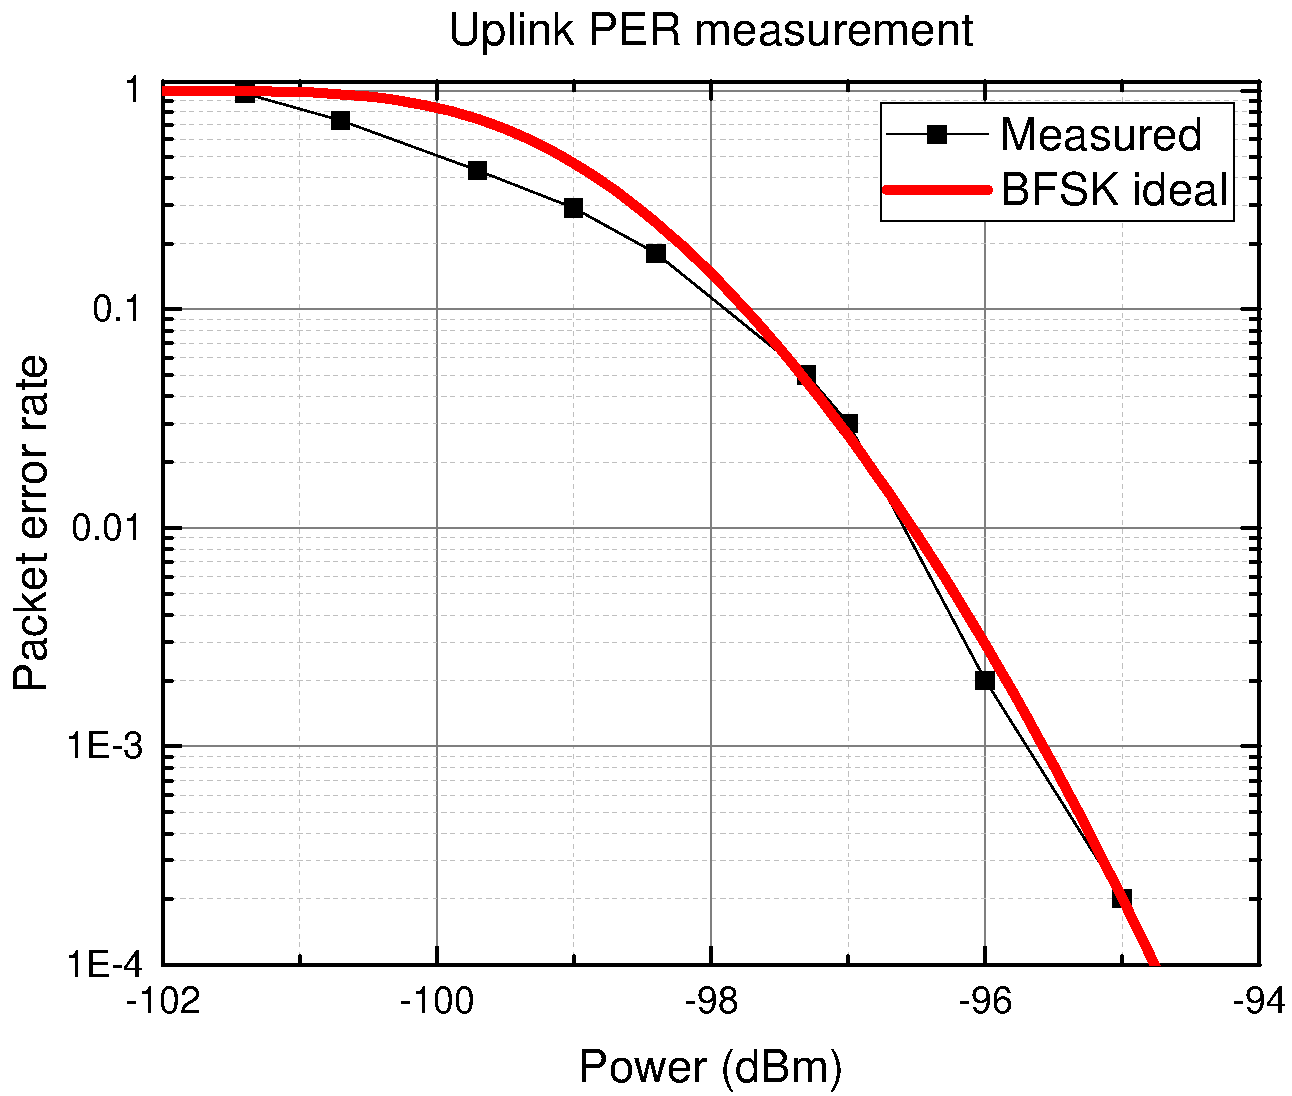
\includegraphics[width=0.8\paperwidth]{img/4/uplink_per.pdf}
    \caption{Uplink sensitivity measurement.}
    \label{4_uplink_sensitivity_graph}
\end{figure}


\subsection{Doppler effect influence on uplink}
Doppler effect is caused when fast-moving object is emitting/receiving radio waves. For uplink frequency (VHF band) Doppler effect influence can shift frequency up to about \SI{5}{\kHz}. The receiver bandwidth should be measured to estimate allowable frequency inaccuracies.

Test setup is the same as in previous setup, shown in the figure \ref{4_uplink_sensitivity}. During the test the PER was measured for a range of frequency offsets from the center frequency of the module. The input power to the module was set to \SI{3}{\dB} above sensitivity level (\SI{-92}{\dBm}) and for each point the number of packets sent was \si{500}.  The result is shown in the chart \ref{TODO}.

\begin{figure}[H]
    \centering
    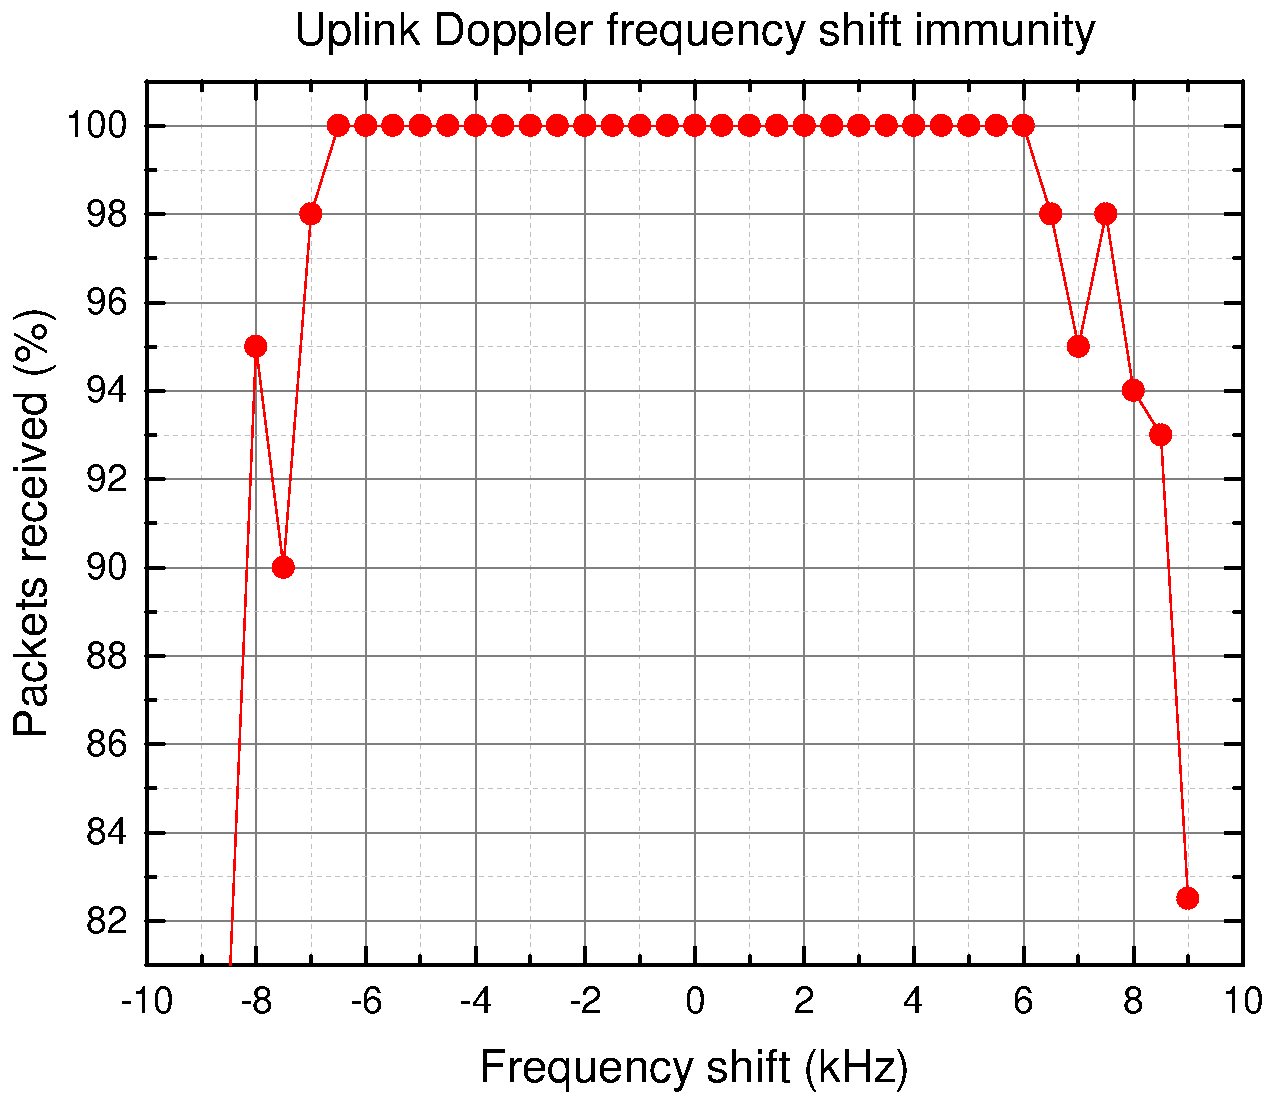
\includegraphics[width=0.6\paperwidth]{img/4/uplink_doppler.pdf}
    \caption{Uplink Doppler effect influence measurement.}
    \label{4_uplink_doppler_measurement}
\end{figure}


\subsection{Transmitter spectrum and output power}
Output power was measured using spectrum analyzer with wide resolution bandwidth. Output power was measured to be \SI{28}{\dBm}, which is in the manufacturers specification.
The spectrum of the signal was recorded, showing significant side lobes (first lobe TODO\SI{10}{\dB} lower than main carrier).
TODO





% -----------------------------------------------------------------------------------------------------------
% -----------------------------------------------------------------------------------------------------------
% -----------------------------------------------------------------------------------------------------------



\section{Spacecraft Antennas}
Because of the selected radio system, two antennas has to be installed - one for uplink (VHF) and one for downlink (UHF). Antennas should be omnidirectional, as PW-Sat2 does not have an nadir-pointing capability and random tumbling during operation is assumed.

Self-made dipole antenna was considered at the design stage, but due to mechanical and time constraints, satellite antenna was decided to be bought as well. Innovative Solutions In Space company sells antenna with with the transceiver as CubeSat communication Kit \texttt{CubeSat dipole antenna system}. Both elements are compatibile and the whole system (transceiver + antenna) is tuned for specific communication frequency and mounting option.

This system is deployable by the command from the on-board computer. Thermal knife (resistor) is heated up and thermal link is burnt, resulting is antenna deploy by the spring action. Antenna is shown in the figure \ref{ISIS_antenna}.

\begin{figure*}
   \centering
\begin{tabular}{cc}
        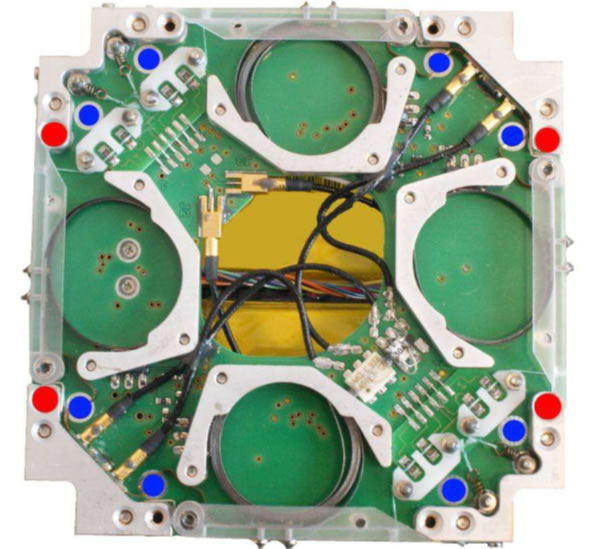
\includegraphics[width=0.3\paperwidth]{img/4/isis_antenna_stowed.jpg}
    & 
        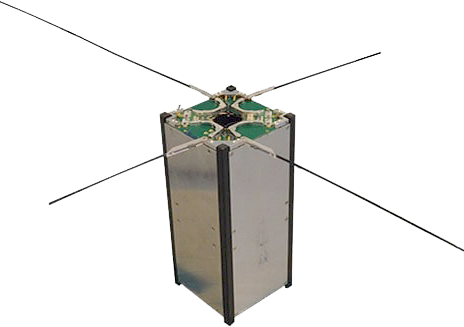
\includegraphics[width=0.45\paperwidth]{img/4/CubeSat-antenna-dipole-configuration.png}    
\end{tabular}
\label{ISIS_antenna}
\caption{ISIS CubeSat dipole antenna system in stowed and deployed position. Source: \cite{isis_dipole_antenna}}
\end{figure*}


\subsection{Measurements}
First automatic task of the satellite it to deploy the antennas. During the test campaign antenna deployment procedure was executed four times, due to the issues with Antenna opening. Satellite during antenna deployment is shown in the figure \ref{pwsat_with_deployed_antennas}.

\begin{figure}[H]
    \centering
    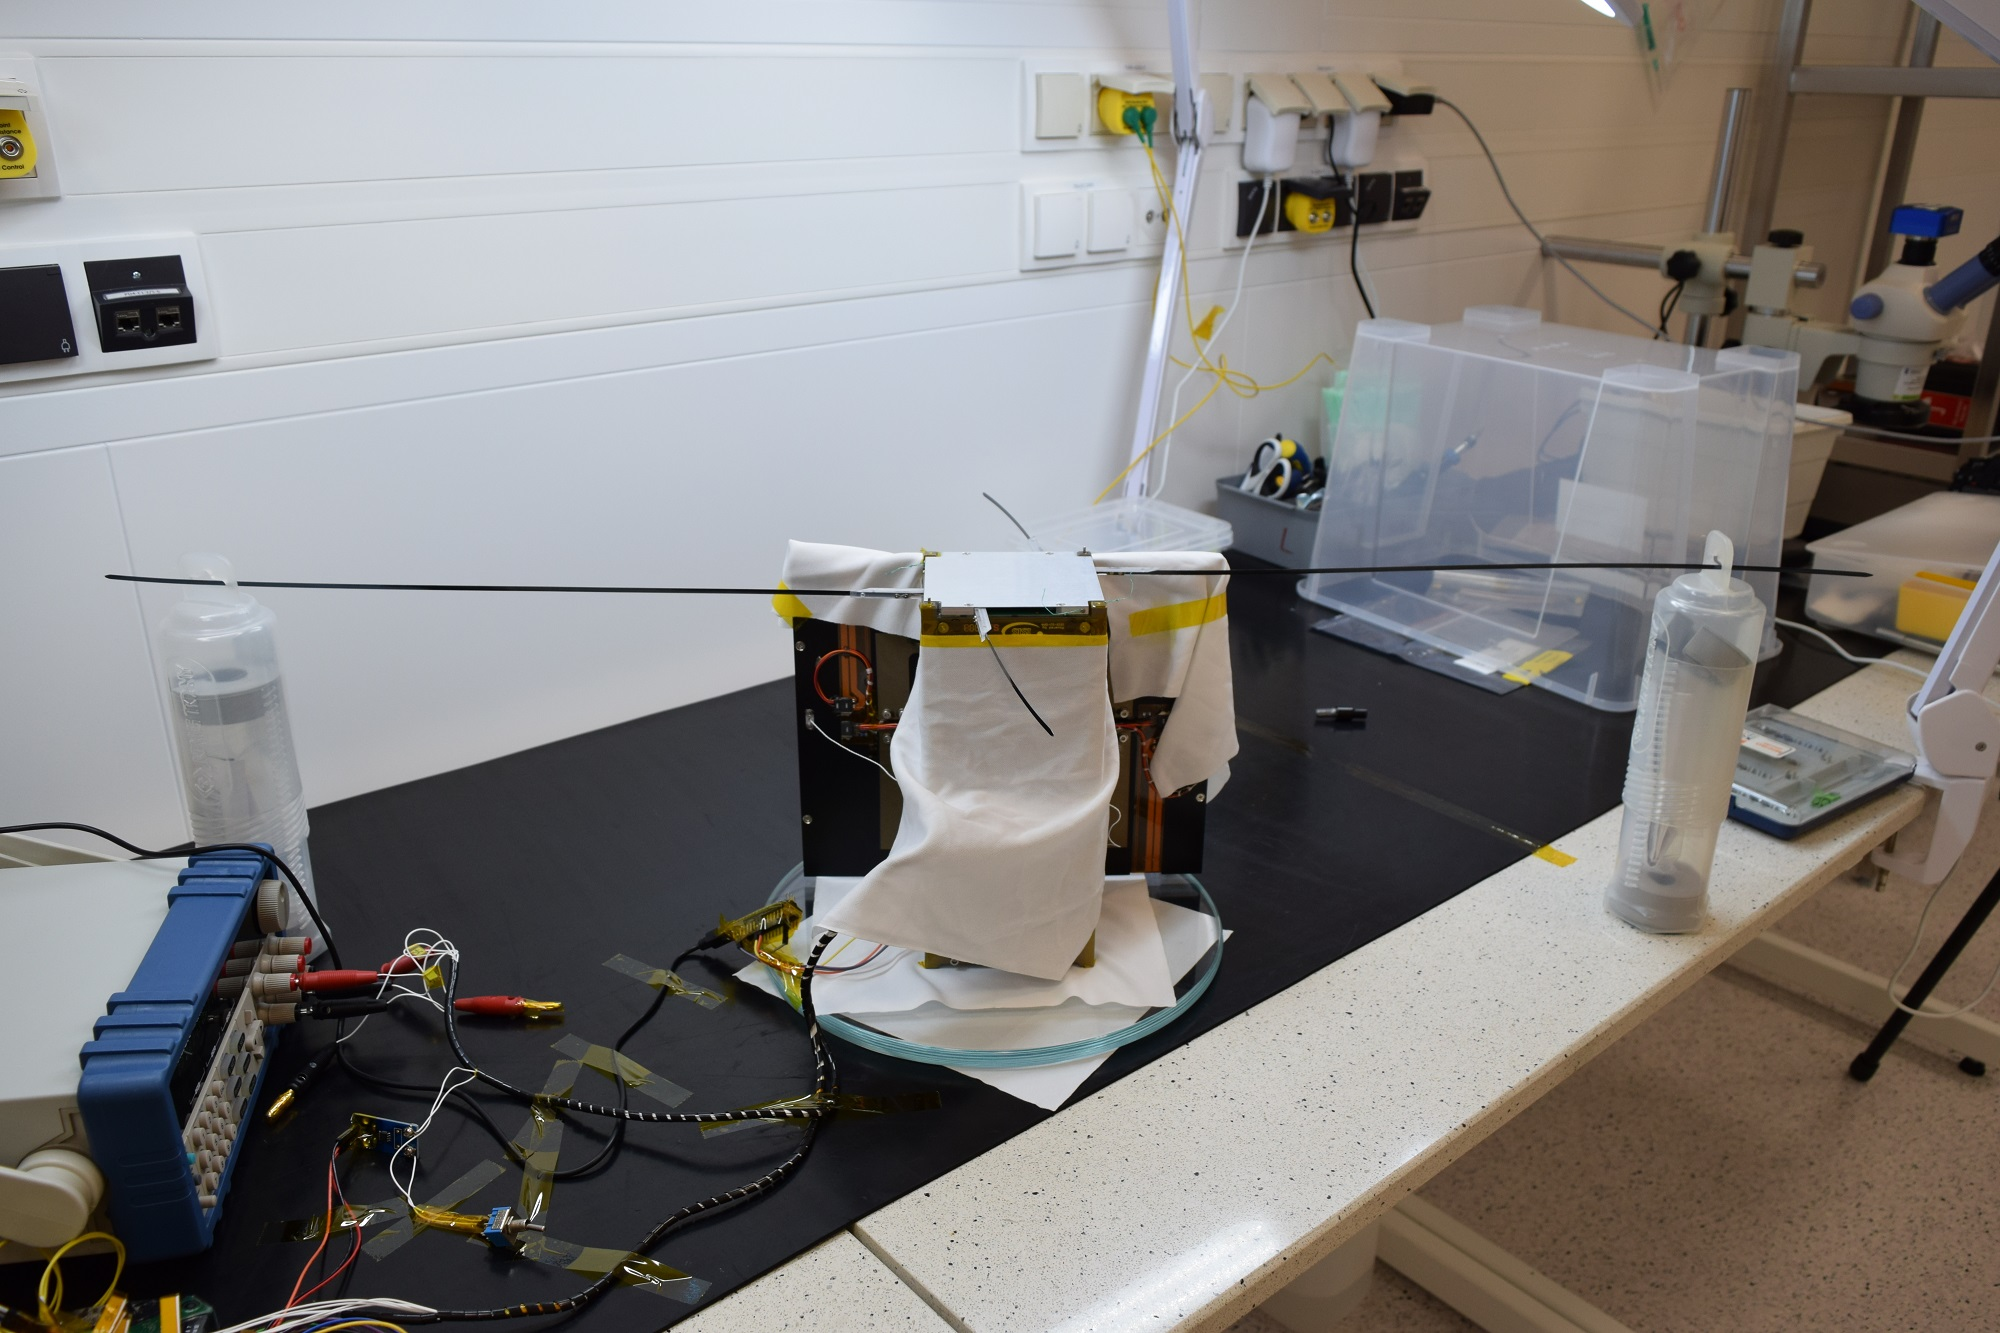
\includegraphics[width=0.6\paperwidth]{img/4/pwsat_with_deployed_antennas.JPG}
    \caption{PW-Sat2 with deployed solar panels during antenna verification.}
    \label{pwsat_with_deployed_antennas}
\end{figure}

Manufacturer of the antennas provide a test report with the measured antennas matchins ($s_{11}$ parameter), for VHF and UHF frequencies they are shown in the figures \ref{isis_s11_vhf} and  \ref{isis_s11_uhf}, respectively.

\begin{figure}[H]
    \centering
    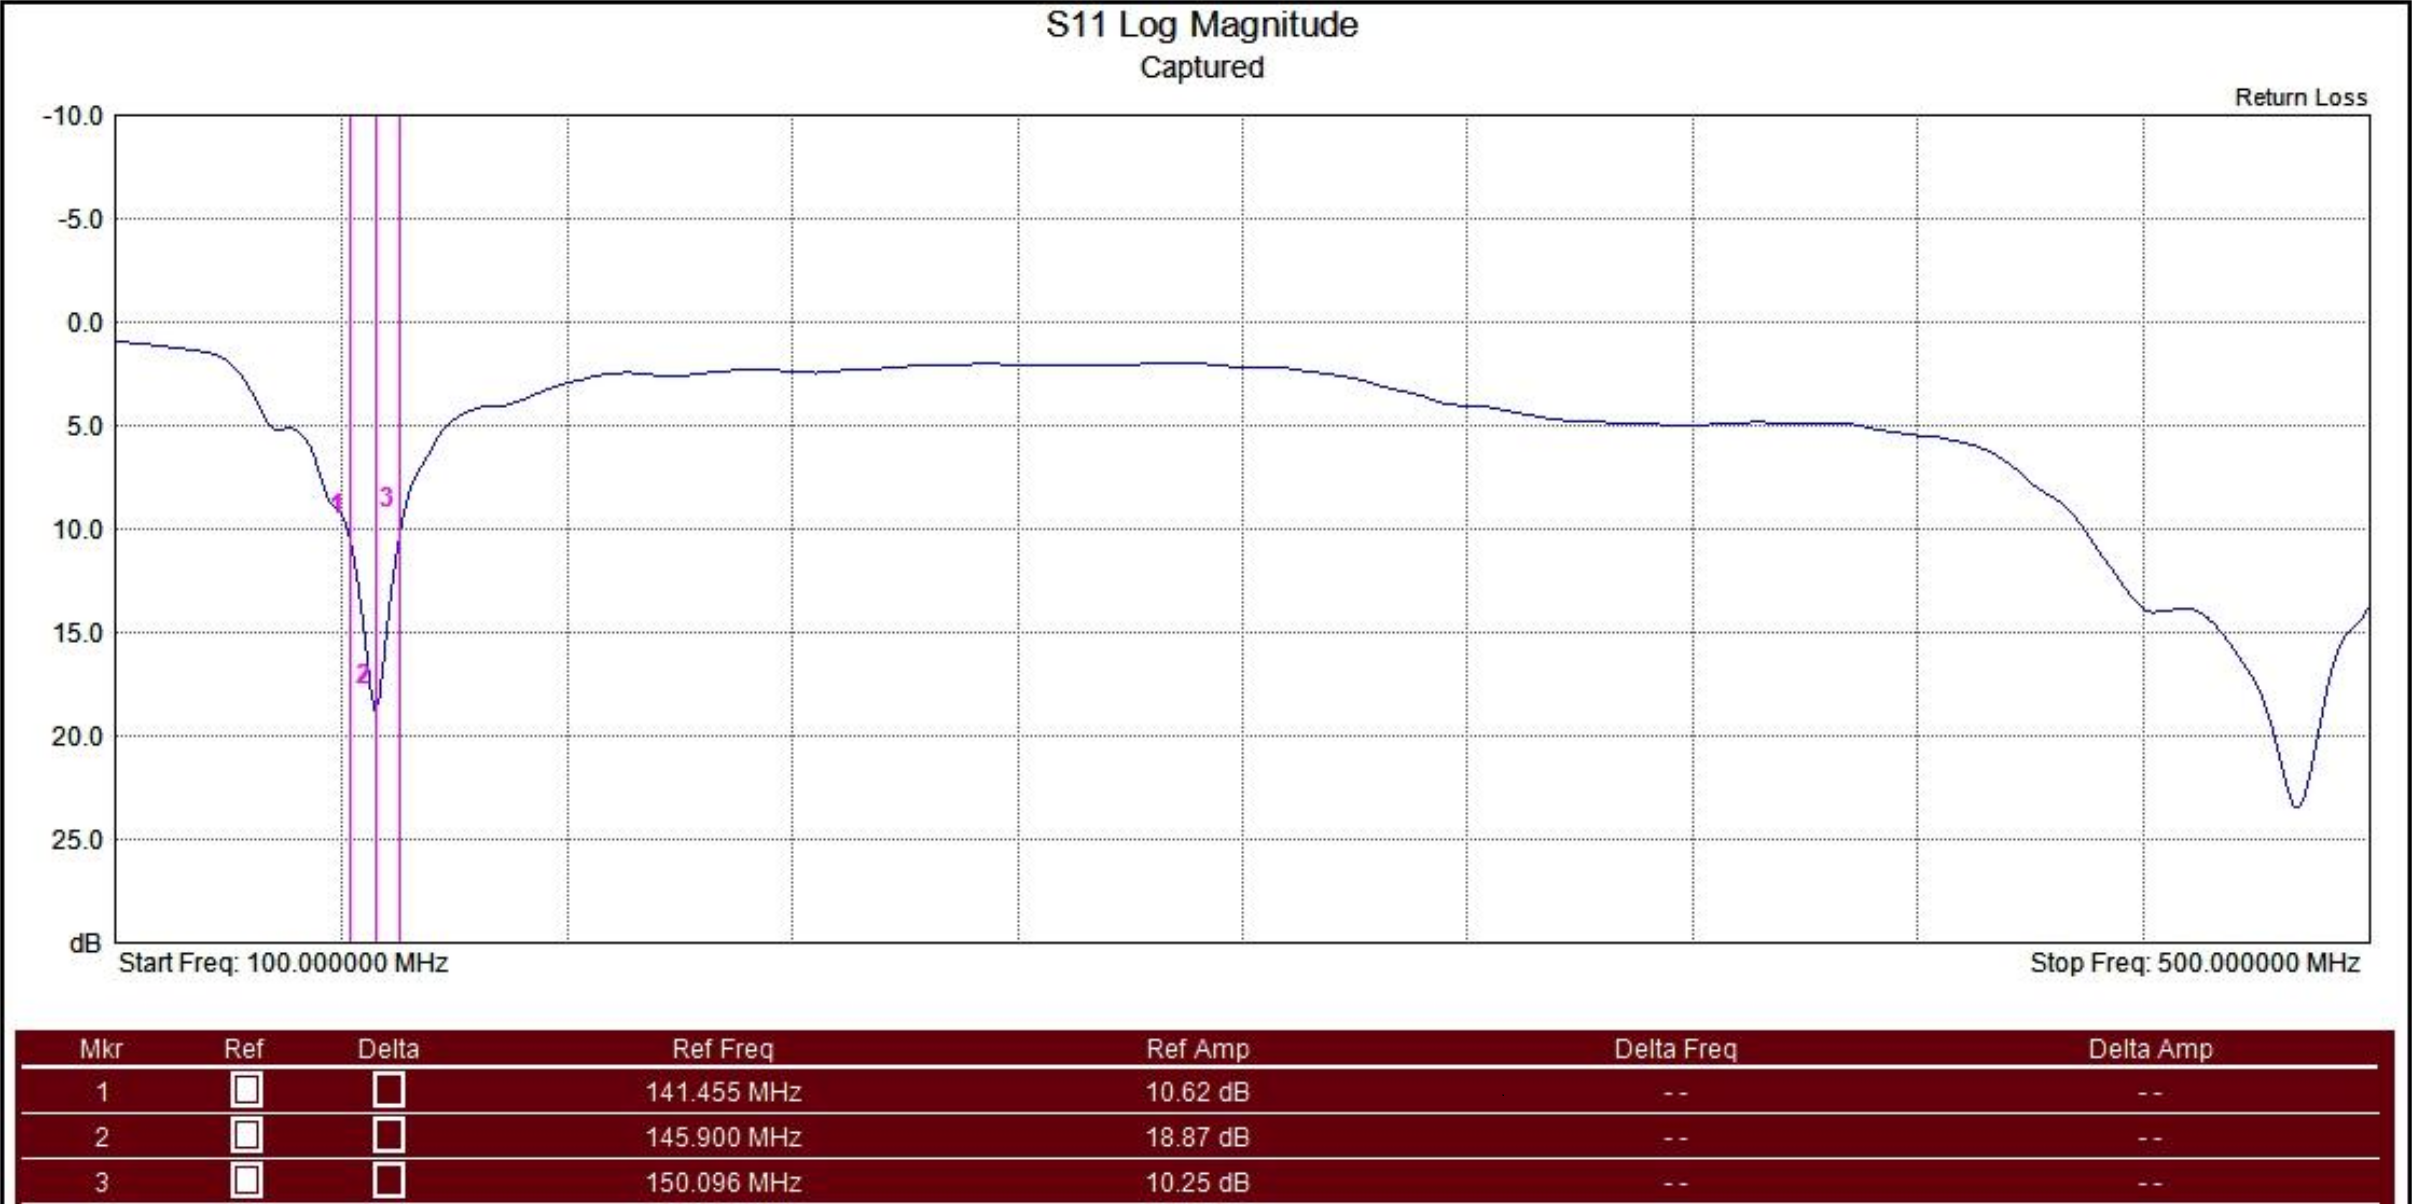
\includegraphics[width=0.8\paperwidth]{img/4/isis_s11_vhf.png}
    \caption{VHF antenna matching.}
    \label{isis_s11_vhf}
\end{figure}

\begin{figure}[H]
    \centering
    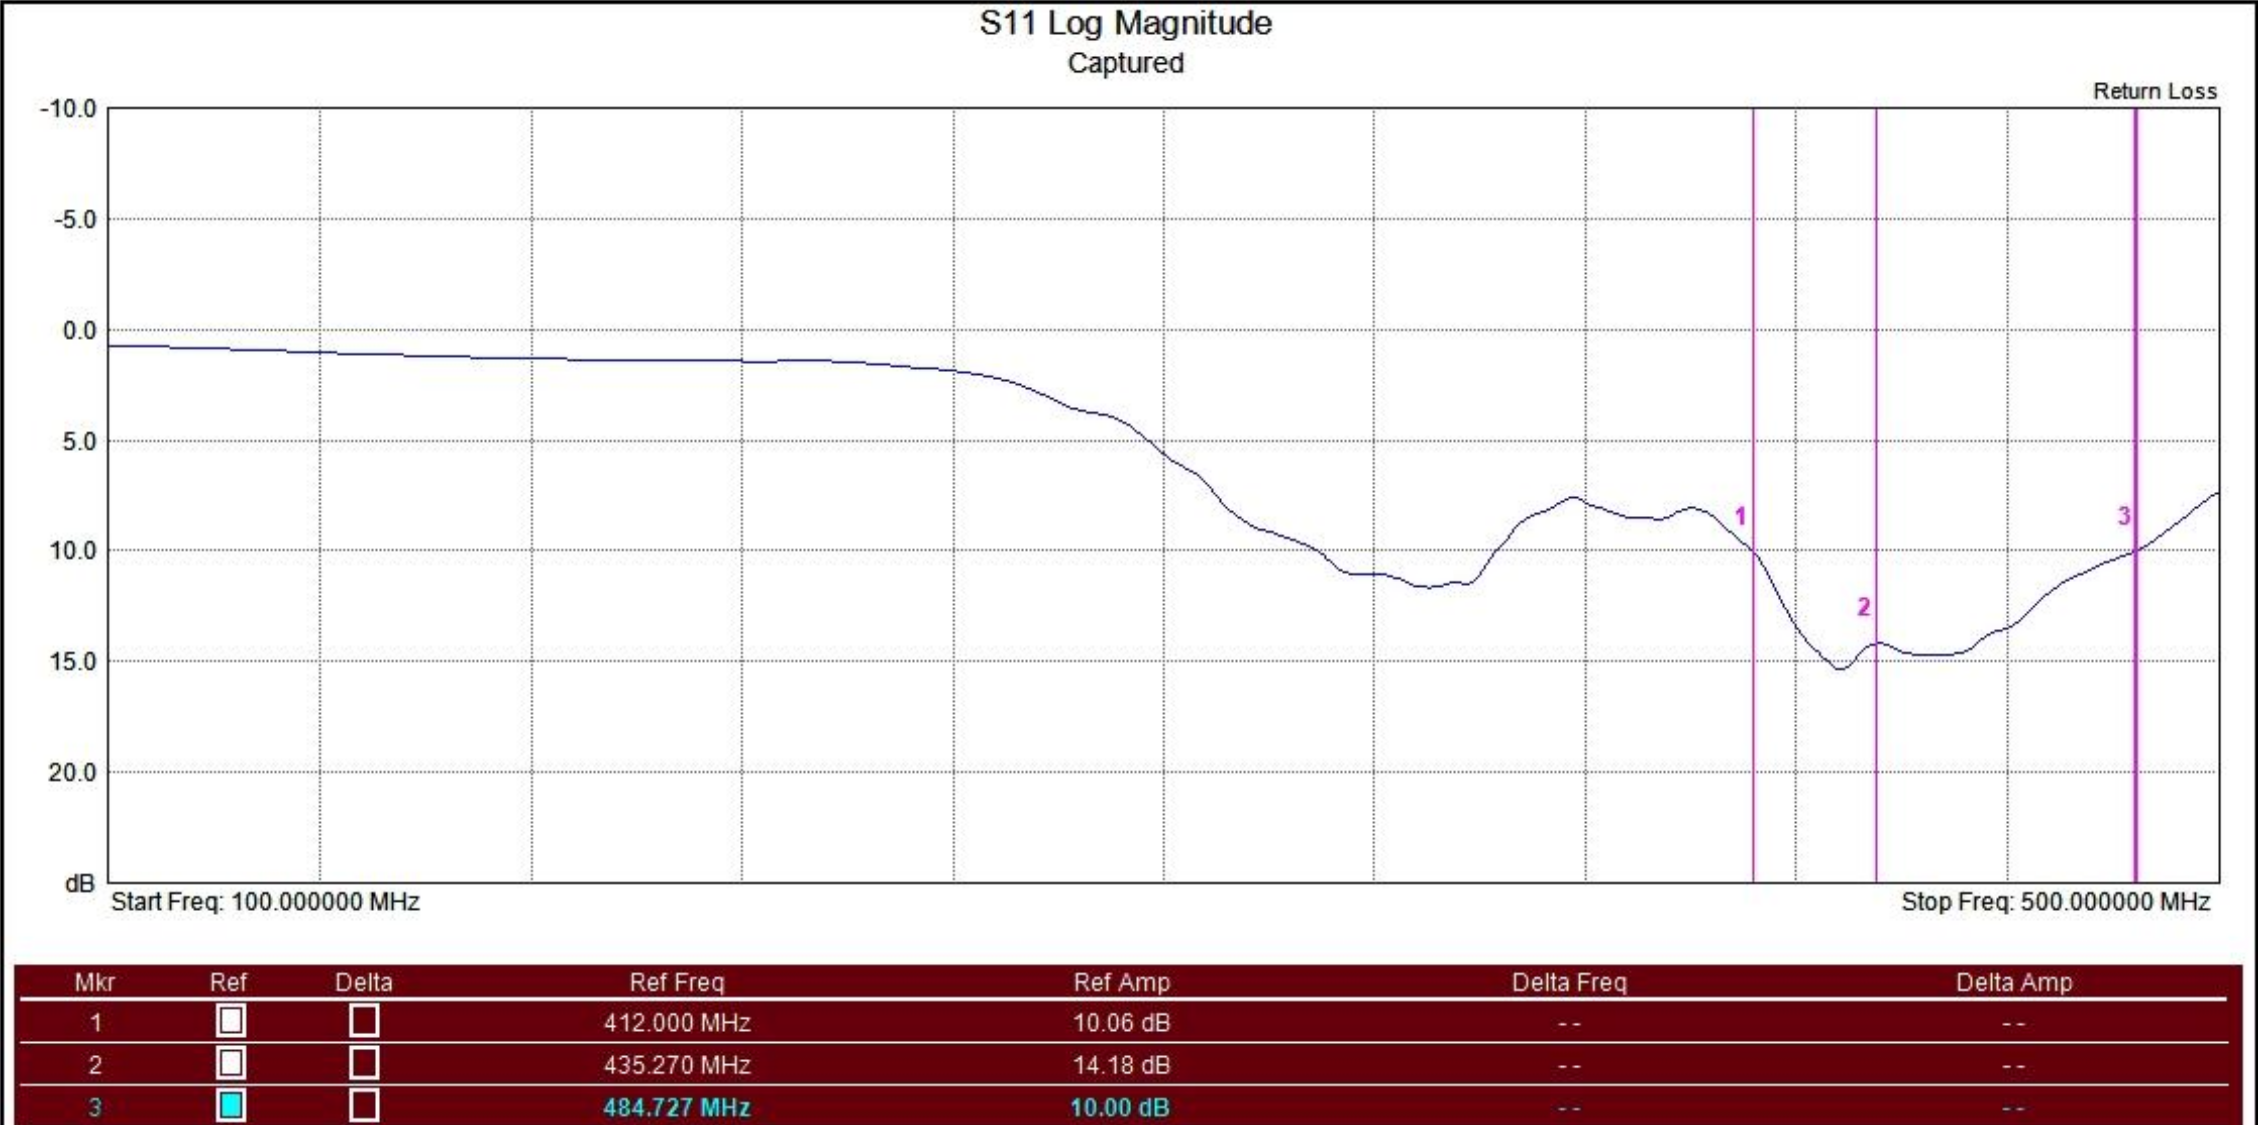
\includegraphics[width=0.8\paperwidth]{img/4/isis_s11_uhf.png}
    \caption{UHF antenna matching}
    \label{isis_s11_uhf}
\end{figure}


Both forward and reflected power from the antenna are measured by the radio module during radio frame transmission. Correct antenna deployment can be verified also by using the telemetry. During the test antenna deployment both forward and reflected power were captured. Average measured value of the forward power: \textbf{\SI{28.8}{\dBm} $\pm$ \SI{0.43}{\dBm}} and reflected power: \textbf{\SI{19.6}{\dBm} $\pm$ \SI{0.54}{\dBm}}. This means that the antenna matching for UHF frequencies is: SWR~$= 2.1$, $s_{11} = -9.2~dB$. This means that the power lost in the mismatch is \SI{0.5}{\dB}. Measured value is similar to measured by the manufacturer ($s_{11} = \SI{-14}{\dB}$).

\subsection{Antennas on orbit}
Reflected and forward power are being captured during the mission, the chart of the reflected and forward power, from the ground testing up to mission completion is shown in the figure \ref{4_rf_power_comm}. This shows that VSWR of the antenna didn't change much during the mission, however Sail and Solar Arrays deploments are clearly seen on the measurements. Picture of the shadow of the satellite on the Sail, showing opened antennas is shown in the figure \ref{antennas_deployed_orbit}.

\begin{figure}[H]
    \centering
    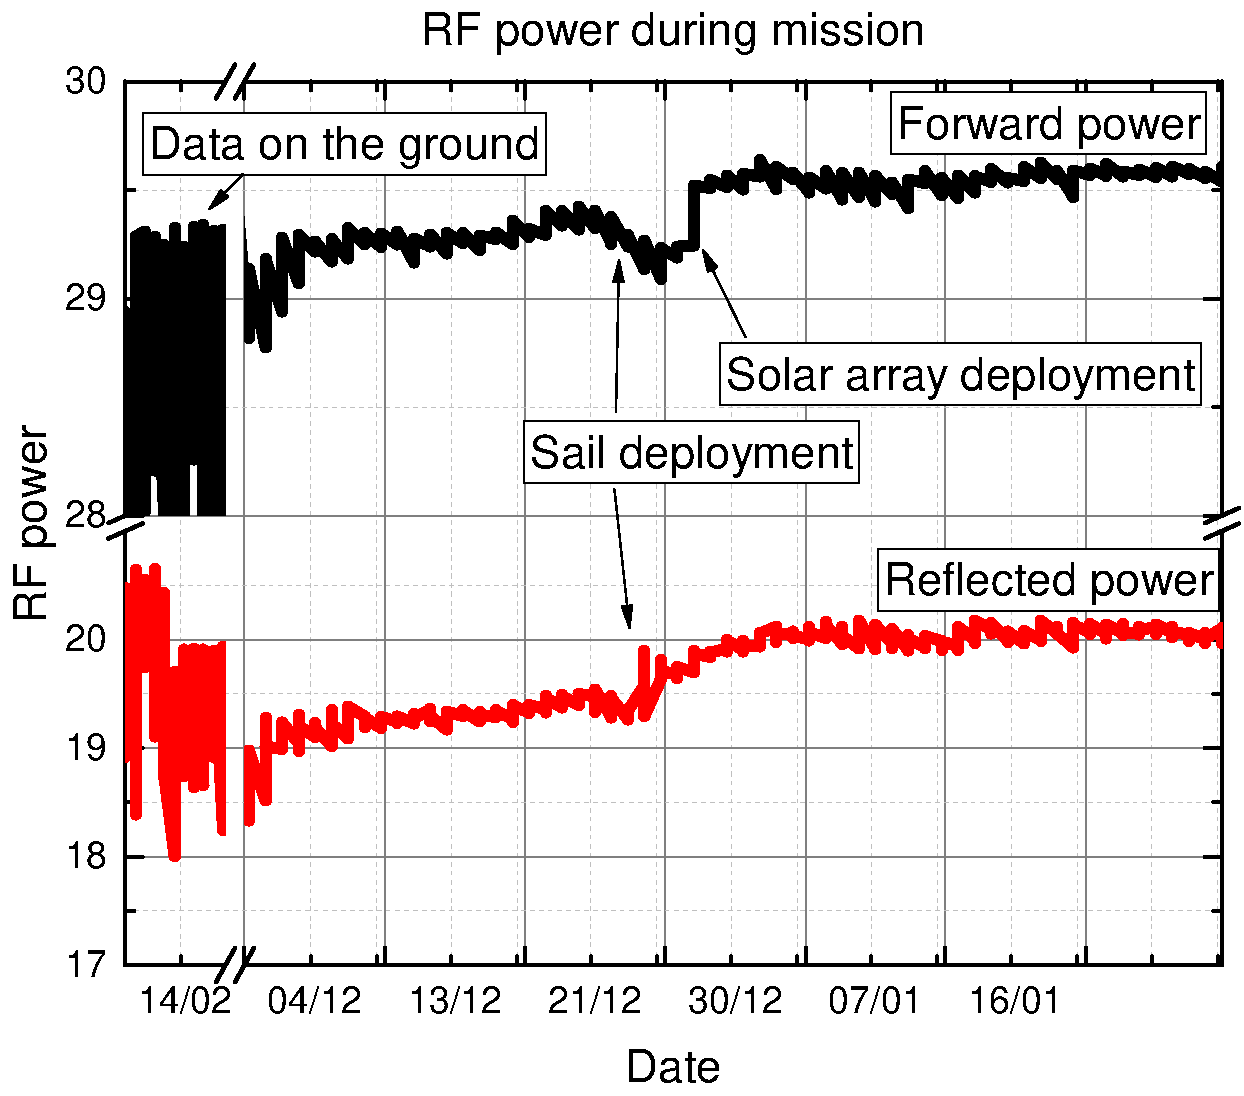
\includegraphics[width=0.6\paperwidth]{img/4/rf_power_comm.pdf}
    \caption{RF power during mission.}
    \label{4_rf_power_comm}
\end{figure}

\begin{figure}[H]
    \centering
    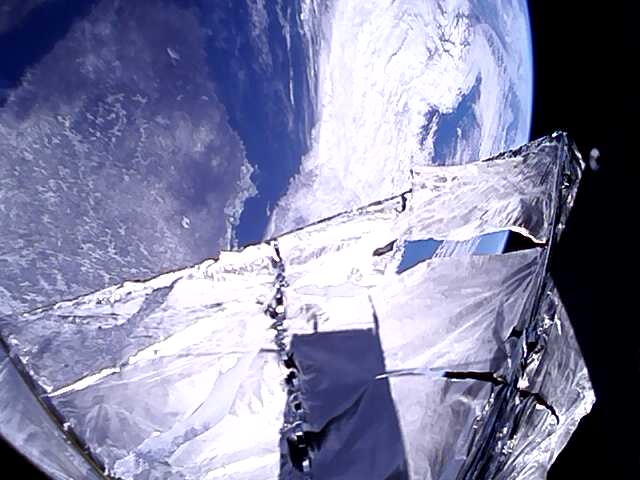
\includegraphics[width=0.7\paperwidth]{img/4/antennas_deployed_orbit.jpg}
    \caption{On-Board photo from PW-Sat2 showing opened antennas.}
    \label{antennas_deployed_orbit}
\end{figure}


% -----------------------------------------------------------------------------------------------------------
% -----------------------------------------------------------------------------------------------------------
% -----------------------------------------------------------------------------------------------------------

% \subsubsection{Deployable elements influence on the antenna pattern}
% TODO

% On-board PW-Sat2 are two main deployables: solar panels and deorbitation sail.

% During design stage, influence of the solar panels was discussed with antenna manufacturer - the outcome was to place longed dipoles (VHF) along the solar panels, and shorter ones orthogonally to it, as shown in the figure \ref{???}

% % TODO: zdjęcie z otwartymi panelami i antenami

% The influence of the deorbit sail was also simulated during Critical Design stage.

% Deorbitation sail is made by very thin (\SI{5}{\micro\meter}) mylar foil with aluminium coating. Using % TODO
% simulation tool, it was shown that the sail will increase directivity of the cubesat antennas, acting as a reflector.
% % TODO: jakieś zdjęcie z symulacji, wynik o ile dB się pogorszyło


